\documentclass{amsart}

%\usepackage[all]{xy}

\usepackage{arxiv}
%\usepackage{ebgaramond}
\usepackage{garamondx}
% \usepackage{CormorantGaramond}

\usepackage[utf8]{inputenc} % allow utf-8 input
\usepackage[T1]{fontenc}    % use 8-bit T1 fonts
\usepackage{hyperref}       % hyperlinks
\usepackage{url}            % simple URL typesetting
\usepackage{booktabs}       % professional-quality tables
\usepackage{amsfonts}       % blackboard math symbols
\usepackage{nicefrac}       % compact symbols for 1/2, etc.
\usepackage{microtype}      % microtypography
% \usepackage{lipsum}		% Can be removed after putting your text content
\usepackage{amsmath} 
\usepackage{amssymb}
\usepackage{graphicx}
\usepackage{epstopdf}
\usepackage{url}
\usepackage{setspace}
\usepackage{amsthm}
\usepackage{mathrsfs}
\usepackage{enumitem}
\usepackage{parskip}
\usepackage{IEEEtrantools}
\usepackage{mathtools}
\usepackage{tensor}
\usepackage{yfonts}
\usepackage{dsfont}
\usepackage{slashed}

%%%%%%%%%%%%%%%%%%% Custom packages
\usepackage{braket}
\usepackage{todo}
\usepackage{xargs}                      % Use more than one optional parameter in a new commands
\usepackage{tikz}
\usepackage{tikz-cd}
\usetikzlibrary{arrows}

%%%% Draft  package and commands %%%%
\usepackage{draft}
%\draftfalse
\newnote{nb}{red}

%%%%%%%%%%%%%%%%%%

\newtheorem{theorem}{Theorem}[section]
\newtheorem{lemma}[theorem]{Lemma}
\newtheorem*{lemma*}{Lemma}
\newtheorem{prop}[theorem]{Proposition}
\newtheorem{corollary}[theorem]{Corollary}
\newtheorem{defn}[theorem]{Definition\rm}
\newtheorem{conjecture}[theorem]{Conjecture}
\newtheorem{remark}{\it Remark\/}
\newtheorem{example}{Example}
\newtheorem{fact}{Fact}

\newcommand{\st}{\ensuremath{:}}% such that
\newcommand{\ie}{\emph{i.e.} }
\newcommand{\eg}{\emph{e.g.} }
\newcommand{\cf}{\emph{cf.} }
\newcommand{\ra}{\rightarrow}
\newcommand{\la}{\leftarrow}
\newcommand{\lra}{\longrightarrow}
\newcommand{\lla}{\longleftarrow}
\newcommand{\lbracket}{\left(}
\newcommand{\rbracket}{\right)}

\newcommand{\al}{\alpha}
\newcommand{\w}{\omega}
\newcommand{\W}{\Omega}
\newcommand{\m}{\mu}
\newcommand{\n}{\nu}
\newcommand{\e}{\epsilon}
\newcommand{\K}{K\"ahler }
\newcommand{\into}{\hookrightarrow}
\newcommand{\PP}{\mathbb{P}}
\newcommand{\RR}{\mathbb{R}}
\newcommand{\CC}{\mathbb{C}}
\newcommand{\QQ}{\mathbb{Q}}
\newcommand{\FF}{\mathbb{F}}
\newcommand{\ZZ}{\mathbb{Z}}
\newcommand{\NN}{\mathbb{N}}
\newcommand{\HH}{\mathbb{H}}
\newcommand{\vp}{\varphi}
\newcommand{\mcA}{\mathcal{A}}
\newcommand{\mcC}{\mathcal{C}}
\newcommand{\mcE}{\mathcal{E}}
\newcommand{\mcF}{\mathcal{F}}
\newcommand{\mcG}{\mathcal{G}}
\newcommand{\mcH}{\mathcal{H}}
\newcommand{\mcL}{\mathcal{L}}
\newcommand{\mcO}{\mathcal{O}}
\newcommand{\mcR}{\mathcal{R}}
\newcommand{\mfg}{\mathfrak{g}}
\newcommand{\mfh}{\mathfrak{h}}
\newcommand{\mfk}{\mathfrak{k}}
\newcommand{\mft}{\mathfrak{t}}
\newcommand{\mc}[1]{\mathcal{#1}}
\newcommand{\mf}[1]{\mathfrak{#1}}
\newcommand{\krr}{k_{\RR}}
\newcommand{\kcc}{k_{\CC}}

\newcommand{\sslash}{\mathbin{/\mkern-6mu/}}
\newcommand{\sssslash}{\mathbin{/\mkern-6mu/\mkern-6mu/\mkern-6mu/}}
\newcommand{\open}[1]{\mathring{#1}}

\newcommand{\pbrackets}[1]{\left( #1 \right)}
\newcommand{\bbrackets}[1]{\left[ #1 \right]}
\newcommand{\norm}[1]{|#1|^{2}}
\newcommand{\tuple}[2]{(#1, \ldots, #2)}
\newcommand{\half}{\frac{1}{2}}
\newcommand{\thalf}{\tfrac{1}{2}}

\newcommand{\dbar}{\overline{\partial}}
\newcommand{\zbar}{\overline{z}}
\newcommand{\wbar}{\overline{w}}
\newcommand{\bmu}{\overline{\mu}}
\newcommand{\mrr}{\mu_{\mathbb{R}}}
\newcommand{\mcc}{\mu_{\mathbb{C}}}
\newcommand{\prr}{\phi_{\mathbb{R}}}
\newcommand{\pcc}{\phi_{\mathbb{C}}}

\DeclareMathOperator{\Lie}{Lie}
\DeclareMathOperator{\Aut}{Aut}
\DeclareMathOperator{\Tr}{Tr}
\DeclareMathOperator{\Image}{Im}
\DeclareMathOperator{\Ad}{Ad}
\DeclareMathOperator{\Diff}{Diff}
\DeclareMathOperator{\Vect}{Vect}
\DeclareMathOperator{\Sympl}{Sympl}
\DeclareMathOperator{\Span}{Span}
\DeclareMathOperator{\ind}{ind}
\DeclareMathOperator{\Td}{Td}
\DeclareMathOperator{\Ch}{Ch}
\DeclareMathOperator{\Ind}{Ind}
\DeclareMathOperator{\pt}{pt}
\DeclareMathOperator{\rk}{rk}
\DeclareMathOperator{\coker}{coker}
\DeclareMathOperator{\Pf}{Pf}
\DeclareMathOperator{\Vol}{Vol}
\DeclareMathOperator{\Res}{Res}
\DeclareMathOperator{\HK}{HK}
\DeclareMathOperator{\cut}{\text{cut}}

\DeclareMathOperator{\Stab}{Stab}

\DeclareMathOperator{\GL}{GL}
\DeclareMathOperator{\SO}{SO}
\DeclareMathOperator{\UU}{U}

\newcommand\restr[2]{{% we make the whole thing an ordinary symbol
		\left.\kern-\nulldelimiterspace % automatically resize the bar with \right
		#1 % the function
		\vphantom{\big|} % pretend it's a little taller at normal size
		\right|_{#2} % this is the delimiter
}}

\title{Geometric Quantisation of Hypertoric Manifolds by Symplectic Cutting}

\date{}	% Here you can change the date presented in the paper title
%\date{} 					% Or removing it

%\author{
%  David S.~Hippocampus\thanks{Use footnote for providing further
%    information about author (webpage, alternative
%    address)---\emph{not} for acknowledging funding agencies.} \\
%  Department of Computer Science\\
%  Cranberry-Lemon University\\
%  Pittsburgh, PA 15213 \\
%  \texttt{hippo@cs.cranberry-lemon.edu} \\
%% examples of more authors
%   \And
% Elias D.~Striatum \\
%  Department of Electrical Engineering\\
%  Mount-Sheikh University\\
%  Santa Narimana, Levand \\
%  \texttt{stariate@ee.mount-sheikh.edu} \\
%% \AND
%% Coauthor \\
%% Affiliation \\
%% Address \\
%% \texttt{email} \\
%% \And
%% Coauthor \\
%% Affiliation \\
%% Address \\
%% \texttt{email} \\
%% \And
%% Coauthor \\
%% Affiliation \\
%% Address \\
%% \texttt{email} \\
%}

\begin{document}
	\maketitle
	
	\begin{abstract}
		Lorem ipsum.
	\end{abstract}
	
	\section{Introduction}
	
	Lorem ipsum.
	
	\section{Background}
    
    \section{Symplectic Toric Manifolds and Orbifolds}
	
    In this section, we shall introduce quickly K\"ahler quotients of $\CC^{n}$ and Delzant's construction of toric manifolds in the smooth case, and Lerman and Tolman's construction of toric orbifolds in the singular case, \cite{Del88, Lerman1997}.
    
    The real torus $T^{n} = \Set{(t_{1}, \ldots, t_{n}) \in \CC^{n} | |t_{i}| = 1 }$ acts diagonally on $\CC^{n}$, preserving its K\"ahler structure, \ie preserving the flat K\"ahler metric and its form,

    \begin{equation}\label{eqn:flat-kahler-form}
        \w = \frac{\sqrt{-1}}{2}\sum_{i=1}^{n} dz_{i} \wedge d\zbar_{i}.
    \end{equation}
    
    The action is Hamiltonian, so it has a moment map which is
    
    \begin{equation}\label{eqn:flat-kahler-moment}
        \phi(z) = \frac{1}{2}\sum_{i=1}^{n}|z_{i}|^{2}e_{i} + \lambda,
    \end{equation}
    
    where the $\{e_{i}\}_{i=1}^{n}$ are the standard basis vectors of $(\mft^{n})^{\ast} \cong \RR^{n}$, and $\lambda \in (\mft^{n})^{\ast}$ is an arbitrary constant. Suppose now that we have a subtorus $K$ of $T^{n}$, with $\dim K = k$, whose Lie algebra $\mfk \subset \mft^{n}$ is generated by rational vectors; with this data, we can perform the symplectic quotient, or even the K\"ahler quotient, with respect to $K$. More precisely, given a collection of non-zero integral vectors $\{u_{1}, \ldots, u_{n}\}$, with each $u_{i} \in \mft^{d}$ where $d= n - k$, which we assume to be primitive and generate $\RR^{d}$.
    
    This data gives rise to the following exact sequence of vector spaces
    
    \begin{equation}\label{eqn:lie-algebra-seq}
        \begin{tikzcd}[ampersand replacement=\&]
            0 \ar[r] \& \mfk \ar[r, hook, "\imath"] \& \mft^{n} \arrow{r}{\pi}[swap]{[u_{1}\ \ldots \ u_{n}]} \& \mft^{d} \ar[r] \& 0,
        \end{tikzcd}
    \end{equation}
    
    and
    
    \begin{equation}\label{eqn:dual-lie-algebra-seq}
        \begin{tikzcd}[ampersand replacement=\&]
            0 \& \ar[l]	(\mfk)^{\ast} \& \ar[l, "\imath^{\ast}", swap] (\mft^{n})^{\ast} \& \arrow{l}[swap]{\pi^{\ast}} (\mft^{d})^{\ast} \& \ar[l] 0,
        \end{tikzcd}
    \end{equation}
    
    where $\pi$ maps $e_{i}$ to $u_{i}$, and $\pi^{\ast}$ is the transpose of its matrix representative. Exponentiating, we also get an exact sequence of abelian groups
    
    \begin{equation}\label{eqn:lie-group-seq}
        \begin{tikzcd}[ampersand replacement=\&]
            1 \ar[r] \& K \ar[r, hook, "\imath"] \& T^{n} \arrow{r}{\pi} \& T^{d} \ar[r] \& 1.
        \end{tikzcd}
    \end{equation}
    
    Depending on the assumptions on the torus $N$, we can either obtain a smooth K\"ahler quotient manifold or a singular K\"ahler quotient orbifold, and these conditions are reflected in the choice of the $u_{i}$. Such choices also analogously determine whether the corresponding hyperk\"ahler quotient is a manifold or an orbifold, when the $u_{i}$ come from the data associated with a polytope in $\RR^{d}$.
    
    The subtorus $K$ acts on $\CC^{n}$ via the inclusion homomorphism $\imath$ into $T^{n}$, hence preserves its flat K\"ahler structure and form (\ref{eqn:flat-kahler-form}). As this $K$-action is also Hamiltonian, it has a moment map which comes from (\ref*{eqn:flat-kahler-moment}),
    
    \begin{equation*}
        \mu(z) = 
    \end{equation*}
    
	\section{Toric Hyperk\"ahler manifolds}
	
	\subsection{Hyperk\"ahler Quotients}
	
	Hyperk\"ahler manifolds are Riemannian manifolds $(M,g)$ with three complex structures $J_{1}, J_{2}$, and $J_{3}$, satisfying the quaternionic multiplication identities, which are compatible with the metric $g$. By compatible we mean that
	\[
		\w_{1}(v,w) = g(J_{1}v,w),\quad \w_{2}(v,w) = g(J_{2}v,w),\quad \w_{3}(v,w) = g(J_{3}v,w),
	\]
	with each $\w_{i}$ a symplectic $2$-form on $M$, so that each quintuple $(M, g, J_{i}, \w_{i})$ constitutes a K\"ahler manifold in their own individual right for $i = 1, 2, 3$; combining these three K\"ahler structures together endows $M$ with a \emph{hyperk\"ahler structure}.
		
	Let us fix a complex structure, $J_{1}$, say. Then the complex-valued $2$-form $\w_{2} + i\w_{3}$ is closed, non-degenerate, and holomorphic with respect to $J_{1}$. Therefore $\w_{\CC} := \w_{2} + i\w_{3}$ is a \emph{holomorphic-symplectic} $2$-form on $M$, and so any hyperk\"ahler manifold can be viewed as a \emph{holomorphic-symplectic} manifold with respect to the complex structure $J_{1}$, real symplectic form $\w_{\RR} := \w_{1}$, and holomorphic symplectic form $\w_{\CC}$.
	
	\begin{example}
		The quaternionic vector space $\HH^{n}$ is a flat hyperk\"ahler manifold whose metric $g$ arises from the Euclidean inner-product on $\RR^{4n}\cong \HH^{n}$, which is K\"ahler with respect to all three complex structures, $J_{1}, J_{2}$, and $J_{3}$ that are identified with $i, j$, and $k$ respectively, via left-multiplication. Fixing the complex structure $J_{1}$ and introducing the coordinates $z_{i} = x_{i} + i y_{i}$ and $w_{i} = u_{i} + i v_{i}$, with $1 \leq i \leq n$, we can identify $\HH^{4n}$ with $\CC^{n} \times \CC^{n}$ via the map
		\[
		x_{i} + iy_{i} + ju_{i} + kv_{i} \mapsto (x_{i} + iy_{i}, u_{i} + iv_{i}).
		\]
		Then the symplectic forms on $\HH^{n}$ are
		\begin{equation*}
			\begin{split}
				\w_{1} &= \sum_{i=1}^{n} dx_{i} \wedge dy_{i} + du_{i} \wedge dv_{i}, \\
				\w_{2} &= \sum_{i=1}^{n} dx_{i} \wedge du_{i} + dv_{i} \wedge dy_{i}, \\
				\w_{3} &= \sum_{i=1}^{n} dx_{i} \wedge dv_{i} + dy_{i} \wedge du_{i}.
			\end{split}
		\end{equation*}
		Recalling that we fixed $J_{1}$, let us write
		\[
		z_{i} = x_{i} + iy_{i}, \quad w_{i} = u_{i} + iv_{i},
		\]
		and express the complex-symplectic form for $\HH^{n}$,
		\[
		\w_{\CC} = \w_{2} + i\w_{3} = \sum_{i=1}^{n} \left( dx_{i} \wedge du_{i} + dv_{i} \wedge dy_{i} \right) + i \left( dx_{i} \wedge dv_{i} + dy_{i} \wedge du_{i} \right) = \sum_{i=1}^{n} dz_{i} \wedge dw_{i}.
		\]
		We can observe now that
		\[
		\w_{\CC} = -d\theta, \quad \text{ where } \quad \theta = \sum_{i=1}^{n} w_{i}dz_{i} \text{ is the canonical symplectic $1$-form for $T^{\ast}\CC^{n}$,}
		\]
		so, after fixing $J_{1}$, we have the identification $(\HH^{n}, \w_{\CC}) \cong (T^{\ast}\CC^{n}, \w_{\text{can}})$.
	\end{example}
	
	
	Given a compact Lie group $G$, we say that an action of $G$ on $M$ is \emph{tri-symplectic} if it preserves each of the symplectic forms $\w_{i}$ which, from the compatibility condition , implies that the action also preserves the metric $g$ and complex structures $J_{i}$; so the action is additionally \emph{isometric} and \emph{tri-holomorphic}. We say that a tri-holomorphic action of $G$ on $M$ is \emph{tri-Hamiltonian} if it is Hamiltonian for each symplectic structure, meaning that there exists three corresponding $G$-equivariant moment maps
	\begin{equation}
		\begin{split}
			\mu_{1}, \mu_{2},\mu_{3} : &M \ra \mfg^{\ast}, \\
			d_{p}\mu_{i}(\xi, X) &= \w_{i}(\xi, X_{p}),\quad \text{at each point } p \in M,
		\end{split}
	\end{equation}
	where $\xi \in T_{p}M$, and $X \in \mfg$. Equivalently, such an action of $G$ on a hyperk\"ahler manifold $M$ is \emph{hyper-Hamiltonian} if it is Hamiltonian with respect to $\w_{\RR}$ and holomorphic Hamiltonian with respect to $\w_{\CC}$, with respective $G$-equivariant moment maps 
	\[
		\mu_{\RR} := \mu_{1} : M \ra \mfg^{\ast}, \quad \text{and} \quad \mu_{\CC} := \mu_{2} + i\mu_{3} : M \ra \mfg_{\CC}^{\ast} \cong \mfg^{\ast} \otimes \CC.
	\]
	
	The moment maps $\mu_{\RR}$ and $\mu_{\CC}$ may then be combined into what we call a \emph{hyperk\"ahler moment map}
	\[
		\mu_{\HK} := \mu_{\RR} \oplus \mu_{\CC} : M \ra \mfg^{\ast} \oplus \mfg_{\CC}^{\ast} \cong \mfg^{\ast} \otimes \RR^{3}.
	\]
	Suppose that $\lambda \in \mfg^{\ast} \oplus \mfg_{\CC}^{\ast}$ is a regular value of $\mu_{\HK}$ and central under the coadjoint action of $G$ on $\mfg^{\ast} \otimes \RR^{3}$, so that $\mu_{\HK}^{-1}(\lambda)$ is a $G$-invariant submanifold of $M$. The \emph{hyperk\"ahler quotient} is defined as
	\[
		M \sssslash_{\lambda}G := \mu_{\HK}^{-1}(\lambda)/G,
	\]
	which also has the structure of a hyperk\"ahler manifold provided that $G$ acts freely on $\mu_{\HK}^{-1}(\lambda)$. Denoting $M_{\lambda} := M \sssslash_{\lambda} G$, when the group $G$ is understood, then: 
	
	\begin{theorem}[\cite{HKLR87}]
		Let $M$ be a hyperk\"ahler manifold equipped with a hyper-Hamiltonian action of a Lie group $G$, and corresponding hyperk\"ahler moment map $\mu_{\HK} : M \ra \mfg^{\ast} \otimes \RR^{3}$. Suppose that $\lambda \in \mfg^{\ast} \otimes \RR^{3}$ is a regular value for $\mu_{\HK}$, and invariant under the coadoint action of $G$. If $G$ acts freely on $\mu_{\HK}^{-1}(\lambda)$, then the hyperk\"ahler quotient $M_{\lambda}$ is a hyperk\"ahler manifold. Moreover, if $G$ is compact and $M$ is complete, then $M_{\lambda}$ is a complete hyperk\"ahler manifold.
	\end{theorem}

	More generally, if $G$ does not act freely on $\mu_{\HK}^{-1}(\lambda)$ but only locally free, then the hyperk\"ahler quotient still has a hyperk\"ahler structure but is a \emph{hyperk\"ahler orbifold} rather than a manifold.
	
	
	
	\subsection{Toric Hyperk\"ahler Manifolds}
	
	Let us quickly go over the construction of toric hyperk\"ahler manifolds; consider the quaternionic vector space $\HH^{n}$, identified with $T^{\ast}\CC^{n}$ after fixing $J_{1}$. The standard linear action of the $n$-dimensional real torus $T^{n}$ induces an action on the cotangent bundle $T^{\ast}\CC^{n}$, and this action is hyper-Hamiltonian. The hyperk\"ahler $T^{n}$-moment map $\mu_{\HK} = \mu_{\RR} + \mu_{\CC}$ on $T^{\ast}\CC^{n}$ is given as follows: let $\{e_{i}\}_{i=1}^{n}$ be the standard basis of the lattice $\mft_{\ZZ}^{n} \subset \mft^{n} \cong \RR^{n}$, and let $\{\e_{i}\}_{i=1}^{n}$ be its dual basis for the dual lattice $(\mft_{\ZZ}^{n})^{\ast} \subset (\mft^{n})^{\ast}$. For $(z,w) = (z_{1},\ldots, z_{n}, w_{1},\ldots w_{n}) \in T^{\ast}\CC^{n}$, where the $z_{i}$ are the base variables of $\CC^{n}$, and $w_{i}$ are the variables of the cotangent fibre, we have
	\begin{align*}%\label{eq:phi-for-Tn}
		\phi_{\RR}(z,w) &= \frac{1}{2} \sum_{i=1}^{n} \left( |z_{i}|^2 - |w_{i}|^2 \right) \e_{i} \in (\mft^{n})^{\ast},
		\mbox{ and}\\
		\phi_{\CC}(z,w) &= \sum_{i=1}^{n} (z_{i} w_{i}) \e_{i} \in (\mft_{\CC}^{n})^{\ast}.
	\end{align*}
	Suppose that $K$ is a $k$-dimensional subtorus of $T^{n}$ whose Lie algebra $\mfk \subset \mft^{n}$ is generated by rational vectors; we wish to take the hyperk\"ahler quotient of $T^{\ast}\CC^{n}$ with respect to the $K$-action induced from the inclusion $\imath : K \ra T^{n}$. Such a subtorus $K$ is determined by a collection of non-zero integral vectors, $\{u_{i}\}_{i=1}^{n}$ in $\mft^{d}$ (where $d = n - k$), which we do not necessarily assume to be primitive, that generate $\mft^{d}$. This data can be represented in the following short exact sequences of vector spaces
	\[
		\begin{tikzcd}[ampersand replacement=\&]
			0 \ar[r] \&
			\mfk \ar[r, hook, "\imath"] \& \mft^{n} \arrow{r}{\pi}[swap]{[u_{1}\ \ldots \ u_{n}]} \& \mft^{d} \ar[r] \& 0,
		\end{tikzcd}
	\]
	and its dualised exact sequence
	\[
		\begin{tikzcd}[ampersand replacement=\&]
			0 \& \ar[l]	(\mfk)^{\ast} \& \ar[l, "\imath^{\ast}", swap] (\mft^{n})^{\ast} \& \arrow{l}{[u_{1}\ \ldots \ u_{n}]^{T}}[swap]{\pi^{\ast}} (\mft^{d})^{\ast} \& \ar[l] 0,
		\end{tikzcd}
	\]
	where $\pi$ sends $e_{i}$ to $u_{i}$. Exponentiating the first exact sequence yields an exact sequence of tori
	\[
		\begin{tikzcd}[ampersand replacement=\&]
			1 \ar[r] \&	K \ar[r, hook, "\imath"] \& T^{n} \arrow{r}{\pi} \& T^{d} \ar[r] \& 1,
		\end{tikzcd}
	\]
	where 
	\[
		T^{n} = \mft^{n}/\mft_{\ZZ}^{n}, \quad T^{d} = \mft^{d}/\mft_{\ZZ}^{d}, \quad \text{ and } \quad K = \ker(\pi : T^{n} \ra T^{d}).
	\]
	Hence $K$ is a compact abelian group with Lie algebra $\mfk$, and is connected (in which case $K$ is a torus) if the vectors $\{u_{i}\}_{i=1}^{n}$ span the lattice $\mft_{\ZZ}^{d}$ over the integers.
	
	Restricting the action of $T^{n}$ on $T^{\ast}\CC^{n}$ to $K$ is hyper-Hamiltonian with hyperk\"ahler moment map
	\[
		\mu_{\HK} = (\imath^{\ast} \circ \phi_{\RR}) \oplus (\imath_{\CC}^{\ast} \circ \phi_{\CC}) : T^{\ast}\CC^{n} \ra \mfk^{\ast} \oplus \mfk_{\CC}^{\ast},
	\]
	where
	\begin{align*}%\label{eq:mu-for-K}
		\mu_{\RR}(z,w) &= \imath^{\ast}\left( \half \sum_{i=1}^{n}(|z_{i}|^{2} - |w_{i}|^{2})\e_{i} \right) \in \mfk^{\ast}
		\mbox{ and}\\
		\mu_{\CC}(z,w) &= \imath_{\CC}^{\ast} \left(\sum_{i=1}^{n}(z_{i}w_{i})\e_{i} \right) \in \mfk_{\CC}^{\ast}.
	\end{align*}
	For an element $\alpha\in \mfk^{\ast}$ and a lift $l = \tuple{l_{1}}{l_{n}} \in (\mft^{n})^{\ast}$, \ie such that $\imath^{\ast}(l) = \lambda$, the K\"ahler quotient
	\[
		X = \CC^{n} \sslash_{\lambda} K = \mu^{-1}(\lambda)/K,
	\]
	is called a \emph{toric variety}, and its hyperk\"ahler analogue
	\[
		M = T^{\ast}\CC^{n} \sssslash_{\lambda} K = \left(\mu_{\RR}^{-1}(\lambda) \cap \mu_{\CC}^{-1}(0)\right)/ K,
	\]
	is called a \emph{hypertoric variety}.
	
    \begin{remark}{Unsure?}
        \break
        When $K$ is not connected, \ie when the vectors $\{u_{i}\}_{i=1}^{n}$ \emph{do not} span $\mft_{\ZZ}^{d}$ over the integers, then $X$ and $M$ are toric and hypertoric \emph{orbifolds} respectively, instead. In this case, $K \cong K_{0} \times \Gamma$, where $K_{0}$ is the connected component of $K$ generated by the identity, hence abelian and so $K_{0}$ is now a torus, whereas $\Gamma$ is a finite abelian group.
    \end{remark}
	
	Suppose for now that $K$ is connected, then both of these have a residual action of $T^{d} = T^{n}/K$ which is effective, and also Hamiltonian in the case of $X$, hyper-Hamiltonian in the case of $M$. Thus $M$ has a residual $T^{d}$ hyperk\"ahler moment map given by
	\begin{align}
		\bmu_{\HK}[z,w] = \bmu_{\RR}[z,w] \oplus \bmu_{\CC}[z,w] &= \half \sum_{i=1}^{n}(|z_{i}|^{2} - |w_{i}|^{2} - l_{i})\e_{i} \oplus \sum_{i=1}^{n}(z_{i}w_{i})\e_{i} \\
		&\in \ker(\imath^{\ast}) \oplus \ker(\imath_{\CC}^{\ast}) \cong (\mft^{d})^{\ast} \oplus (\mft_{\CC}^{d})^{\ast}.
	\end{align}

	Its image is surjective onto $(\mft^{d})^{\ast}$, divided up into polyhedra by a hyperplane arrangement.

	\subsection{Hyperplane Arrangements}
	
	The data used to construct a hypertoric orbifold $M$, consisting of the collection of non-zero vectors $\{u_{i}\}$ in $(\mft^{d})^{\ast}$ and an element $\lambda \in \mfk^{\ast}$, can be encoded into a finite \emph{hyperplane arrangement} in $(\mft^{d})^{\ast} \cong \RR^{d}$. 
	
	\begin{defn}
		Let $H \subseteq \RR^{d-1}$ be a (linear) hyperplane in $\RR^{d}$, \ie for $u \in \RR^{d}$ a non-zero fixed vector, that
		\[
			H = \Set{x \in \RR^{d} | \langle x,\, u \rangle = 0 }.
		\]
		Then:
		\begin{enumerate}
			\item[(rational) --] The hyperplane $H$ is \emph{rational} if $u$ has integer-valued components, \ie $u \in \ZZ^{d}$.
			\item[(weighted) --] The hyperplane $H$ is \emph{weighted} if $u$ is not required to be primitive.
			\item[(cooriented) --] Observe that the linear hyperplane $\bar{H} = \Set{ x \in \RR^{d} | \langle x,\, -u \rangle = 0}$ defines the same codimension-$1$ subspace of $\RR^{d}$ as $H$.  A \emph{coorientation} is a choice of sign for the vector $u$, and a hyperplane $H$ is \emph{cooriented} if it has a coorientation.
			\item[(affine) --] A hyperplane $\tilde{H}$ is \emph{affine} if it is a translate of the linear hyperplane $H$,
			\[
				\tilde{H} = \Set{x \in \RR^{d} | \langle x,\, u \rangle = a,\, a \in \RR} \subseteq \RR^{d-1}.	
			\]
		\end{enumerate}
	\end{defn}

	Applied to our case, the collection of vectors $\{u_{i}\}$ in $\mft^{d}$ and choice of lift $\lambda \in (\mft^{n})^{\ast}$ with $\alpha = \imath^{\ast}(\lambda)$ correspond to a hyperplane arrangement $\mcA = \{H_{1}, \ldots, H_{n}\}$ of rational, weighted, cooriented, affine hyperplanes $H_{i}$ in $(\mft^{d})^{\ast}$, given by
	\[
		H_{i} = \Set{ x \in (\mft^{d})^{\ast} | \langle x,\, u_{i} \rangle = \lambda_{i}}.
	\]
	Observe that if we choose a different lift $\tilde{\lambda} \in (\mft^{n})^{\ast}$ such that $\tilde{\lambda} -\lambda \in \ker(\imath^{\ast})$, then this corresponds to a translation of the arrangement $\mcA$ inside of $(\mft^{d})^{\ast}$, and is represented geometrically by shifting the K\"ahler and hyperk\"ahler moment maps by $\tilde{\lambda} - \lambda \in \ker(\imath^{\ast}) = (\mft^{d})^{\ast}$. 
	
	A hyperplane $H_{i}$ gives rise to the following two half-spaces in $(\mft^{d})^{\ast}$
	\begin{align*}
		H_{i}^{+} &= \Set{ x \in (\mft^{d})^{\ast} | \langle x,\, u_{i} \rangle \geq \lambda_{i} }, \\
		H_{i}^{-} &= \Set{ x \in (\mft^{d})^{\ast} | \langle x,\, u_{i} \rangle \leq \lambda_{i} },
	\end{align*}
	determined by their cooriented normal vector $u_{i}$, and clearly $H_{i} = H_{i}^{+} \cap H_{i}^{-}$.
	
	Let
	\[
		\Delta = \bigcap_{i=1}^{n} H_{i}^{+} = \Set{x \in (\mft^{d})^{\ast} | \langle x,\, u_{i} \rangle \geq \lambda_{i}, \text{ for each } 1 \leq i \leq n }.
	\]
	be the polytope in $(\mft^{d})^{\ast}$ determined by the hyperplane arrangement $\mcA$; it is the image under $\bar{\mu}_{\RR}$ of the K\"ahler toric variety $X = \CC^{n}\sslash_{\alpha} K$.
	
	\subsection{Examples}
	
	In this subsection, we shall introduce some examples of the above construction for hypertoric manifolds and orbifolds.
	
	\subsubsection{$M = T^{\ast}\CC\PP^{2}$}
	
	Here, we consider
	\[
		u_{1} = (1,0), \quad u_{2} = (0,1), \quad u_{3} = (-1,-1),
	\]
	so that
	\[
		\pi = \begin{bmatrix}
			1 & 0 & -1 \\ 0 & 1 & -1
		\end{bmatrix},
		\quad \text{ and } \quad
		\imath = \begin{bmatrix}
			1 & 1 & 1
		\end{bmatrix}^{T},
		\quad \text{ so } \quad
		\imath^{\ast} = \begin{bmatrix}
			1 & 1 & 1
		\end{bmatrix}.
	\]
	They fit into the exact sequence of Lie algebras,
	\[
	\begin{tikzcd}[ampersand replacement=\&]
		0 \ar[r] \&
		\mfk \ar[r, hook, "\imath"] \& \mft^{3} \arrow{r}{\pi} \& \mft^{2} \ar[r] \& 0,
	\end{tikzcd}
	\]
	that exponentiates to
	\[
	\begin{tikzcd}[ampersand replacement=\&]
		0 \ar[r] \&
		K \ar[r, hook, "\imath"] \& T^{3} \arrow{r}{\pi} \& T^{2} \ar[r] \& 0.
	\end{tikzcd}
	\]
	From $\imath : K \hookrightarrow T^{3}$, which is $t \mapsto (t,t,t)$, we see that the moments map for this $K$-action are
	\begin{align*}
		(\imath^{\ast} \circ \mu_{\RR})(z,w) &= \frac{1}{2}\left(|z_{1}|^{2} +|z_{2}|^{2} +|z_{3}|^{2} - |w_{1}|^{2} - |w_{2}|^{2} - |w_{3}|^{2} \right) - (\lambda_{1} + \lambda_{2} + \lambda_{3}) \in \mfk^{\ast}, \\
		(\imath_{\CC}^{\ast} \circ \mu_{\CC})(z,w) &= z_{1}w_{1} + z_{2}w_{2} + z_{3}w_{3} \in \mfk_{\CC}^{\ast},
	\end{align*}
	so that
	\begin{align*}
		(\imath^{\ast} \circ \mu_{\RR})^{-1}(0) &= \Set{(z,w) \in T^{\ast}\CC^{n} | \tfrac{1}{2}\left(\|z\|^{2} - \|w\|^{2} \right) = \lambda_{1} + \lambda_{2} + \lambda_{3}}, \\
		(\imath_{\CC}^{\ast} \circ \mu_{\CC})^{-1}(0) &= \Set{(z,w) \in T^{\ast}\CC^{n} | \langle z,\, w \rangle = 0 }.
	\end{align*}
	Let us set $(\lambda_{1}, 0, 0) = (\alpha, 0, 0)$, whence
	\[
		M_{\alpha} = T^{\ast}\CC^{3} \sssslash_{\alpha} K \cong T^{\ast}\CC\PP^{2}.
	\]
	There is a residual $T^{2}$-action on $M_{\alpha}$, that is hyperHamiltonian and whose real moment map image is shown in Figure (\ref{fig:TCP2-moment-image}):
	
	\begin{figure}[h!]
		\centering
		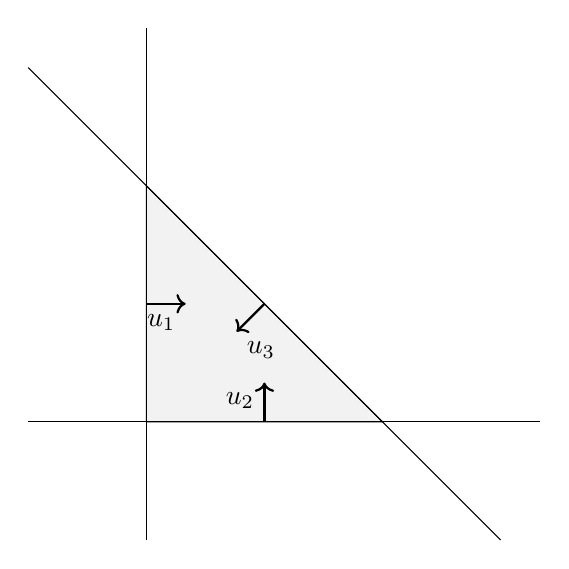
\begin{tikzpicture}
			\filldraw[fill=gray!10!white, draw=black] (0,0) -- (3,0) -- (0,3) -- cycle;
			\draw (-1.5,0) -- (5,0);
			\draw[thick,->] (1.5,0) -- (1.5,0.5) node[anchor=north east] {$u_{2}$};
			\draw (0,-1.5) -- (0,5);
			\draw[thick,->] (0,1.5) -- (0.5,1.5) node[anchor=north east] {$u_{1}$};
			\draw (4.5,-1.5) -- (-1.5,4.5);
			\draw[thick,->] (1.5,1.5) -- (1.146,1.146) node[anchor=north west] {$u_{3}$};
		\end{tikzpicture}
		\caption{Image of $T^{\ast}\CC\PP^{2}$ under $\mu_{\RR}$ in $(\mft^{2})^{\ast}$ for the $T^{2}$-action. The shaded $2$-simplex is the image of the core, $\mcE \cong \CC\PP^{2}$.} \label{fig:TCP2-moment-image}
	\end{figure}
		
	\subsection{The Core, Extended Core, and Residual $S^{1}$-Action}
	
	In general, the hyperplane arrangement $\mcA = \{H_{1}, \ldots, H_{n} \}$ divides $(t^{d})^{\ast}$ into a finite family of closed, convex polyhedra, indexed by subsets $A \subseteq \{1,\ldots, n\}$,
	\[
	\Delta_{A} = \left(\bigcap_{i \not\in A} H_{i}^{+} \right) \cap \left(\bigcap_{i \in A} H_{i}^{-} \right).
	\]
	For each subset $A \subseteq \{1, \ldots, n\}$, set
	\[
	\mcE_{A} = \bar{\mu}_{\RR}^{-1}(\Delta_{A})\cap \bar{\mu}_{\CC}^{-1}(0).
	\]
	Each $\mcE_{A} \subseteq M$ is a K\"ahler suborbifold of $M$ with respect to $\w_{\RR}$, and is the (not necessarily compact) K\"ahler symplectic toric orbifold associated to $\Delta_{A}$ with an effective Hamiltonian $T^{d}$-action, in its own right. Let
	\[
		I := \Set{A \subseteq \{1, \ldots, n\} | \Delta_{A} \text{ is bounded}},
	\]
	be the set of subsets of $\{1, \ldots, n\}$. We call the \emph{core} of $M$ the union
	\[
		\mcC := \bigcup_{A \in I} \mcE_{A}.
	\]
	
	There is a residual Hamiltonian $S^{1}$-action on each hypertoric manifold $M$, descending from an action of $S^{1}$ on the cotangent bundle $T^{\ast}\CC^{n}$ by rotating the fibres with weight $1$, \ie
	\[
		t\cdot (z,w) = (z,tw).
	\]
	It is Hamiltonian with respect to the real K\"ahler form, $\w_{\RR}$, and restricts to the trivial action on the zero section $\CC^{n}$, hence this $S^{1}$-action is trivial on $X$.
	
	The complex-symplectic moment map $\mu_{\CC} : T^{\ast}\CC^{n} \ra (\mft_{\CC})^{d})^{\ast}$ is $S^{1}$-equivariant with respect to this action and the scalar multiplication of $S^{1}$ of $(\mft_{\CC^{n}})^{\ast}$,
		\[
		\mu_{\CC}\left(t\cdot(z,w)\right) = \mu_{\CC}(z,tw) = \sum_{i=1}^{n}\left(z_{i}(tw_{i})\right)e_{i} = t\mu_{\CC}(z,w),
		\]
	therefore $S^{1}$ preserves the level-set $\mu_{\CC}^{-1}(0)$. 
	
	Define the \emph{extended core}
	\[
		\mcE := \Set{[z,w] \in M | z_{i}w_{i} = 0, \text{ for all } i },
	\]
	and the \emph{extended core components}, already introduced in the previous subsection,
	\[
		\mcE_{A} = \bar{\mu}_{\RR}^{-1}(\Delta_{A})\cap \bar{\mu}_{\CC}^{-1}(0) = \Set{[z,w] \in M | w_{i} = 0, \text{ if } i \not\in A, \text{ and } z_{i} = 0, \text{ if } i \in A}.
	\]
	\begin{lemma}
		If $w_{i} = 0$, then $\Image(\bar{\mu}_{\RR}) \subseteq H_{i}^{+}$. If $z_{i} = 0$, then $\Image(\bar{\mu}_{\RR}) \subseteq H_{i}^{-}$.
	\end{lemma}
	
	\begin{proof}
		Set
		\[
			(T^{\ast}\CC^{n})_{A} = \Set{(z,w) \in T^{\ast}\CC^{n} | w_{i} = 0, \text{ if } i \not\in A, \text{ and } z_{i} = 0, \text{ if } i \in A} \subset T^{\ast}\CC^{n},
		\]
		and consider the following hyperplane arrangement $\tilde{\mcA} = \{ \tilde{H}_{1}, \ldots, H_{n}\}$ in $(\mft^{n})^{\ast}$, determined by the following half-spaces in $(\mft^{n})^{\ast}$
		\begin{align*}
			\tilde{H}_{i}^{+} &= \Set{ y \in (\mft^{n})^{\ast} | \langle y,\, e_{i} \rangle \geq \lambda_{i} }, \\
			\tilde{H}_{i}^{-} &= \Set{ y \in (\mft^{n})^{\ast} | \langle y,\, e_{i} \rangle \leq \lambda_{i} }, \\
			\tilde{H}_{i} &= \tilde{H}_{i}^{+} \cap \tilde{H}_{i}^{-}.
		\end{align*}
		Recall
		\[
			\mu_{\RR}(z,w) = \frac{1}{2}\sum_{i=1}^{n}\left(|z_{i}|^{2} - |w_{i}|^{2} - \lambda_{i} \right)e_{i},
		\]
		thus, restricted to $(T^{\ast}\CC^{n})_{A}$, its image in $(\mft^{n})^{\ast}$ is
		\begin{align*}
			\Image\left(\restr{\mu_{\RR}}{(T^{\ast}\CC^{n})_{A}} \right) =& \left(\bigcap_{i \not\in A} \tilde{H}_{i}^{+}\right) \cap \left(\bigcap_{i \in A} \tilde{H}_{i}^{-}\right) \\
			=& \Set{x \in (\mft^{n})^{\ast} | \langle x,\, e_{i} \rangle \geq \lambda_{i}, \text{ if } i \not\in A } \\
			&\cap \Set{x \in (\mft^{n})^{\ast} | \langle x,\, e_{i} \rangle \leq \lambda_{i}, \text{ if } i \in A } .
		\end{align*}
		Call this image $\tilde{\Delta}_{A}$ then, as $\pi^{\ast}$ is injective, $\pi^{\ast}\Delta_{A} \cong \tilde{\Delta}_{A}$. Now for $x \in (\mft^{n})^{\ast}$, we have $\imath^{\ast}(x) = 0 \iff x = \pi^{\ast}(y)$, for some $y \in (\mft^{d})^{\ast}$, and
		\begin{align*}
			&\langle \pi^{\ast}(y),\, e_{i} \rangle \geq \lambda_{i}, \text{ for all } i \not\in A, \\
			\text{and } \quad  &\langle \pi^{\ast}(y), \, e_{i} \rangle \leq \lambda_{i}, \text{ for all } i \in A,
		\end{align*}
		which implies
		\begin{align*}
		\langle y,\, \pi_{\ast}(e_{i}) \rangle &= \langle y,\, u_{i} \rangle \geq \lambda_{i}, \text{ for all } i \not\in A, \\
		\text{and } \quad  \langle y,\, \pi_{\ast}(e_{i}) \rangle &= \langle y,\, u_{i} \rangle \leq \lambda_{i}, \text{ for all } i \in A.
		\end{align*}
		Specialising now to the case $\mu_{\RR}(z,w) = x$, and $\bar{\mu}_{\RR}[z,w] = y$, we have that $\bar{\mu}_{\RR}[z,w] \in H_{i}^{+}$ if $i \not\in A$, and $\bar{\mu}_{\RR}[z,w] \in H_{i}^{-}$ if $i \in A$.
	\end{proof}

	\begin{lemma}
		Each extended core component $\mcE_{A}$ is isomorphic to the $d$-dimensional symplectic toric variety whose moment polytope is $\Delta_{A}$.
	\end{lemma}

	Globally, the $S^{1}$-action does not act as a subtorus of $T^{d}$ on $M$. However, when restricted to a extended core component $\mcE_{A}$, $S^{1}$ does act on $\mcE_{A}$ as a subtorus of $T^{d}$, and its inclusion $\jmath : S^{1} \hookrightarrow T^{d}$ depends on the subset $A \subseteq \{1, \ldots, n\}$ in a combinatorial fashion.
	Suppose $[z, w] \in \mcE_{A}$, then for $t \in S^{1}$
	\[
		t \cdot [z, w] = [z, tw] = [z_{1}, \ldots, z_{n}, tw_{1}, \ldots, tw_{n}] = [t_{1}z_{1}, \ldots, t_{n}z_{n}, t_{1}^{-1}w_{1}, \ldots, t_{n}^{-1}w_{n}], \text{ where } t_{i} =
		\begin{cases}
			t^{-1}, &\text{ if } i \in A, \\
			1, &\text{ if } i \not\in A,
		\end{cases}
	\]
	which holds because $t_{i} = t^{-1}$ when $z_{i} =0$, and $t_{i} = 1$ when $z_{i} \neq 0$.
	This determines how $S^{1}$ can be viewed as a subtorus of the original torus $T^{n}$, and the image of this subtorus under the mapping $\pi$ is how $S^{1}$ acts on each $\mcE_{A}$ via a codimensional-$1$ subtorus of the residual torus $T^{d}$. On the Lie algebra level, this inclusion is the composition
	\[
	\begin{tikzcd}[ampersand replacement=\&]
		\mf{s} \arrow[r, "\jmath_{A}"] \&
		\mft^{n} \arrow[r, "\pi"] \& \mft^{d}, \& \& 1 \arrow[r, mapsto] \& -\sum_{i \not\in A}e_{i} \arrow[r, mapsto] \& -\sum_{i \not\in A} u_{i},
	\end{tikzcd}
	\]
	where $\jmath_{A} : \mf{s} \ra \mft^{n}$ is the derivative of the inclusion homomorphism, arising from the above discussion. As it acts as a subtorus, the $S^{1}$-action is effective and Hamiltonian, and its moment map globally is just
	\[
		\Phi : M \ra \mf{s}^{\ast}, \quad [z,w] \mapsto \frac{1}{2}\|w\|^{2}, \text{ (plus some constant in } (\mf{s}^{\ast})\text{)}.
	\]
	Restricted to each component $\mcE_{A}$ however, as $S^{1}$ acts via the inclusion $\jmath_{A}$ into $T^{n}$, its restricted moment map is
	\[
		\restr{\Phi}{\mcE_{A}}[z,w] = (\jmath_{A}^{\ast} \circ \mu_{\RR})[z,w] = \left\langle \bar{\mu}_{\RR}[z,w], \, -\sum_{i \in A} u_{i} \right\rangle = \left\langle \mu_{\RR}(z,w), \, -\sum_{i \in A} e_{i} \right\rangle.
	\]
	For brevity relabel $\restr{\Phi}{\mcE_{A}}$ as $\Phi_{A}$, viewed as the moment map map $\Phi_{A} : \mcE_{A} \ra \mf{s}^{\ast}$.
	
	\section{Symplectic Toric and Hypertoric Suborbifolds}
	
	\subsection{Symplectic Toric Suborbifolds}
	
	We recall the definition of a symplectic toric orbifold.
	
	\begin{defn}{\cite{Aud04,Lerman1997}}
		A $2n$-dimensional \emph{symplectic toric orbifold} is a connected symplectic orbifold $(M, \w)$ equipped with an effective Hamiltonian action of a $n$-torus $T^{n}$ and with corresponding moment map $\mu : M \ra (\mft^{n})^{\ast}$.
	\end{defn}

	We also have the orbifold analogue to the Delzant construction \cite{Del88}, where each symplectic toric orbifold can be associated to a labelled polytope.
	
	\begin{defn}{\cite{Lerman1997}}
		A \emph{labelled polytope} in $\RR^{n}$ is a convex rational simple polytope $\Delta$ such that $\dim\Delta = n$, along with a positive integer attached to each facet.
	\end{defn}

	\begin{theorem}{\cite{Lerman1997}}
		\begin{enumerate}\label{thm:orbifold-characterisation}
			\item To every compact symplectic toric orbifold $(M, \w, T^{n}, \mu)$ there naturally corresponds a labelled polytope: the image of the moment map $\mu(M)$ is a rational simple polytope, $\Delta$. For every open facet $\open{F}$ of $\Delta$ there exists a positive integer $n_{\open{F}}$ such that the structure group of every $x \in \mu^{-1}(\open{F})$ is $\ZZ/n_{\open{F}}\ZZ$.
			\item Two compact symplectic toric orbifolds are isomorphic if and only if their associated labelled polytopes are isomorphic.
			\item Every labelled polytope arises from some compact symplectic toric orbifold.
		\end{enumerate}
	\end{theorem}

	\begin{remark}
		Theorem (\ref{thm:orbifold-characterisation}), due to Lerman and Tolman, is the orbifold analogue of Delzant's construction for toric symplectic manifolds. Since orbifolds will appear naturally in this article, and also as a manifold is a special case of an orbifold, we consider the more general notion of an orbifold in this section. However, these results also apply to manifolds; one just needs to strengthen the simple condition on the respective polytope to being in fact a \emph{smooth} one meaning that, for each vertex of a polytope in $\RR^{n}$, the normals to the edges emanating from it form an integral basis for $\ZZ^{n}$.
	\end{remark}
	
	Now let $(M, \w, G, \mu)$ be an $2n$-dimensional symplectic toric orbifold, where $G$ is a torus acting in an effective and Hamiltonian way on $M$, with associated moment map $\mu : M \ra \mfg^{\ast}$ under which the image of $M$ is a convex and simple polytope $\Delta_{G}$. Then we have the following result:
	
	\begin{prop}\label{thm:fixed-point-suborbifold}
		For a subtorus $H \lhd G$, the fixed-point set $M^{H}$ in $M$ is a symplectic orbifold.
	\end{prop}
	
    There are a finite number of subtori $H_{i}$ which can appear as stabiliser subgroups of points in $M$, with each fixed-point set having a finite number of components. Denote the set of these components by $\mcF = \{F_{1}, \ldots, F_{n} \}$, and label their respective stabiliser subtori by $\{H_{1}, \ldots, H_{n}\}$.
    
    By Proposition (\ref{thm:fixed-point-suborbifold}), each of these fixed-point components is a symplectic orbifold in its own right. Moreover, restricting the moment map $\mu$ to each $F_{i}$ makes it into a Hamiltonian $G$-space, albeit with a non-effective action. We obtain an effective Hamiltonian action of the quotient torus $T_{i} = G/H_{i}$ however, though the moment map for it is only unique up to a translate (\ie up to a constant) in $\mfg^{\ast}$.
    
    In the case when the quotient subtori $T_{i}$ has codimension $1$ in $G$, \ie when $H_{i}$ is a circle, then the corresponding fixed-point component $F_{i}$ also has codimension $1$ in $M$. In this case, the image of the moment map $\mu$, restricted to $F_{i}$, is an $(n-1)$-dimensional face $\Delta_{i}$ of $\Delta_{G}$, namely a facet. This facet $\Delta_{i}$ has a respective normal vector, $u_{i} \in \mfg$, and it is this normal vector that generates the Lie algebra of the stabiliser subgroup of $F_{i}$ in $G$, that is
    \[
    	\mfh_{i} = \Span_{\RR}\Set{u_{i} | u_{i} \text{ is normal to } \Delta_{i}} \subset \mfg, \quad \text{ and } \quad H_{i} \cong \Stab_{G}(F_{i}) \lhd G.
    \]
    
   \subsection{Below - Old Content} 
    
	Suppose that
	\[
		\Delta_{G} = \bigcap_{i=1}^{n} \Set{x \in \mfg^{\ast} | \langle x,\, u_{i} \rangle \geq \lambda_{i} },
	\]

    where the $u_{i} \in \mfg$ are the inwards-pointing normal vectors to the half-spaces that delineate the polytope, and each $\lambda_{i} \in \mathbb{R}$. Let $\mcF = \{ F_{1}, \ldots, F_{n}\}$ be the set of faces of $\Delta_{G}$, \ie codimension $1$ subpolytopes of $\Delta_{G}$; each $F_{i}$ can be described by the condition
    \[
        F_{i} = \Set{ x \in \mfg^{\ast} | \langle x,\, u_{i} \rangle = \lambda_{i} }.
    \]
    Since $\Image(\mu) \subseteq \mfg^{\ast}$ and $u_{i} \in \mfg$, we can consider the component of the moment map in the $u_{i}$ direction, namely
    \[
        \mu_{i} : M \ra \RR, \quad \mu_{i}(z,w) := \langle \mu(z,w),\, u_{i} \rangle, \text{ for each } 1 \leq i \leq n.
    \]
    Set $\tilde{F}_{i} := \mu_{i}^{-1}(\lambda_{i}) \subset M$, so that $\mu_{i}(\tilde{F}_{i}) = F_{i}$. Then $\tilde{\mcF} = \{\tilde{F}_{1}, \ldots, \tilde{F}_{n}\}$ are the fixed-point components in $M$, themselves being symplectic orbifolds. Each of their stabilisers $H_{i} := \Stab_{G}(\tilde{F}_{i})$ is generated by the respective normal vector $u_{i}$, in the sense that
    \[
    	\mfh_{i} = \RR\cdot u_{i}, \quad \text{so that} \quad H_{i} = \Set{\exp(t\cdot u_{i}) | t \in \RR}.
    \]
    
    Each fixed-point component $\tilde{F}_{i} \subset M$ has codimension $1$, though there are higher codimension fixed-point components constructed from taking intersections of the $\tilde{F}_{i}$. Namely, for some subset $I \subseteq \{1, \ldots, n\}$ with $|I| = d$, the intersection $\tilde{F}_{I} := \cap_{i \in I} \tilde{F}_{i}$ has codimension $d$ in $M$. Moreover, its stabiliser is the subtorus generated by the Lie algebra
    \[
    	\mfh_{I} = \Span_{\RR}\Set{u_{i} | i \in I}, \quad \text{ so that } H_{I} = \prod_{i=1}^{d}\Set{\exp(t_{1}\cdot u_{i}) | t_{i} \in \RR }.
    \]
    	
	\section{Localisation and Symplectic Cutting}
	
	\subsection{Orbifold Dolbeault Complex}
	
	Let $(M, \w)$ be a compact symplectic manifold, and assume that the class of the symplectic form is integral, \ie $[\w] \in H^{2}(M; \ZZ)$. This condition implies existence of a Hermitian line bundle $\mcL \ra M$, whose $1$\textsuperscript{st} Chern class is $c_{1}(\mcL) = [\w]$; then It is then possible to choose a Hermitian connection $\nabla$ on $\mcL$ with curvature form $F(\mcL) = (2\pi/i)\w$. In the case when $M$ is moreover K\"ahler, which we shall assume, then the line bundle $\mcL$ can be taken to be holomorphic. The complex structure $J$ induces a Dolbeault structure on the exterior algebra of the cotangent bundle, giving rise to a splitting of the complexified tangent bundle of $M$ into the $+i$ and $-i$ eigenspaces of $J$,
    \[
        TM \otimes \CC \cong T^{1,0}M \oplus T^{0,1}M.
    \]
    The exterior powers of the complexified tangent bundle also split, giving a bigrading,
    \[
        \wedge^{k}T^{\ast}M \otimes \CC \cong \bigoplus_{i + j = k} \wedge^{i,j},
    \]
    and the $k$-th order differential forms $\Omega^{k}(M)$ also decomposes according to their form type:
    \[
        \Omega^{k} = \bigoplus_{i + j = k}\Omega^{i,j}.
    \]
    Let $d$ be the de Rham exterior derivative, and $\pi^{i,j} : \Omega^{\ast}(M) \ra \Omega^{i,j}(M)$ denote the projection onto the $(i,j)$-type forms. Set
    \[
        \dbar = \pi^{0,j+1} \circ d : \Omega^{0,j} \ra \Omega^{0,j+1}.
    \]
    When $M$ is a complex analytic orbifold, the operator $\dbar$ defines the \emph{Dolbeault orbifold complex},
    \[
        \begin{tikzcd}[ampersand replacement=\&]
            0 \ar[r] \& \Omega^{0,0} \ar[r, "\dbar"] \& \Omega^{0,1} \ar[r, "\dbar"] \& \ldots \ar[r, "\dbar"] \& \Omega^{0,n} \ar[r] \& 0.
        \end{tikzcd}
    \]
    Now, given the holomorphic line bundle $\mcL$ from before with its holomorphic connection $\nabla$, we define a \emph{twisted Dolbeault complex} by setting $\dbar_{\mcL} = \dbar \otimes 1 + 1 \otimes \nabla$, which defines the following complex for $\mcL$-valued forms
    \[
    \begin{tikzcd}[ampersand replacement=\&]
        0 \ar[r] \& \Omega^{0,0} \otimes \mcL \ar[r, "\dbar_{\mcL}"] \& \Omega^{0,1} \otimes \mcL \ar[r, "\dbar_{\mcL}"] \& \ldots \ar[r, "\dbar_{\mcL}"] \& \Omega^{0,n} \otimes \mcL \ar[r] \& 0.
    \end{tikzcd}
    \]
    The cohomology of this complex is the sheaf cohomology of holomorphic sections of $\mcL$,
    \[
        \ker \dbar_{\mcL}^{0,j} / \Image \dbar_{\mcL}^{0,j-1} \cong H^{j}(M, \mcO(\mcL)).
    \]
    From $\w$ and $J$, we also have a Hermitian structure of each of the $\Omega^{0,j}$'s, so that the adjoint operator $\dbar_{\mcL}^{\ast}$ is well-defined. The operator $\slashed{\partial}_{\CC} = \dbar_{\mcL} + \dbar_{\mcL}^{\ast}$ is known as the spin-$\CC$ Dirac operator and, as $M$ is compact, the spaces $\ker \slashed{\partial}_{\CC}$ and $\coker \slashed{\partial}_{\CC}$ are finite-dimensional; the difference $\dim \ker \slashed{\partial}_{\CC} - \dim \coker \slashed{\partial}_{\CC}$ is equal to the \emph{index} of the spin-$\CC$ Dirac operator, $\slashed{\partial}_{\CC}$:
    \[
        \Ind \slashed{\partial}_{\CC} := \dim \ker \slashed{\partial}_{\CC} - \dim \coker \slashed{\partial}_{\CC}.
    \]
	
    The Atiyah-Singer Index Theorem expresses this index as the integral over $M$ of the product of the Todd class of the tangent bundle to $M$, and the Chern character of $\mcL$,
    \[
        \Ind \slashed{\partial}_{\CC} = \int_{M} \Td(TM) \cdot e^{c_{1}(\mcL)}.
    \]	
    
    \subsubsection{Index Theorems for Orbifolds}
    
    

	\subsection{Symplectic Cutting}
	
	Here, we introduce the symplectic cutting operation of Lerman \cite{Ler95}, which we shall use to compactify our hypertoric manifolds using the residual Hamiltonian circle action, by performing the cut on each extended core component $\mcE_{A}$. As this action depends on the subset $A \subset \{1, \ldots, n\}$ determining $\mcE_{A}$, we shall see that the cut itself does too. This results in a compactified hypertoric orbifold, with the compactification reflected in the image of the real moment map by slicing through each $\Delta_{A}$ with a inwards-pointing half-space, whose normal vector depends on the subset $A$.
	
	Before applying symplectic cuts to our hypertoric orbifolds, let us quickly introduce the main ideas.
	
	\paragraph{General Symplectic Cutting}
	
	Let $(M,\w)$ be a symplectic manifold with a Hamiltonian circle action, with moment map $\mu : M \ra \RR$. Now consider the product $M \times \CC$, with the product symplectic structure and diagonal $S^{1}$-action,
	\[
		e^{i\theta} \cdot (m, \xi) \longmapsto (e^{i\theta} \cdot m, e^{i\theta}\xi), \quad (m,\xi) \in M \times \CC,
	\]
	with moment map
	\[
		\rho : M \times \CC \ra \RR, \qquad \rho(m,\xi) = \mu(m) + \frac{1}{2}|\xi|^{2}.
	\]
	
	\begin{defn}
		The \emph{symplectic cut} $M^{\leq\e}$ of $M$ is the symplectic reduction of the product $M \times \CC$ at level $\e$ with respect to the diagonal $S^{1}$-action,
		\[
			M^{\leq\e} := (M \times \CC) \sslash_{\e} S^{1} = \rho^{-1}(\e)/S^{1}.
		\]
	\end{defn}
	
	In \cite{Ler95}, Lerman shows that the level-set
	\[
		\rho^{-1}(\e) = \Set{(m, \xi) \in M \times \CC | \mu(m) + \tfrac{1}{2}|\xi|^{2} = \e}
	\]
	is the same as the disjoint union $\Sigma_{1} \sqcup \Sigma_{2}$, where
	\begin{align*}
		\Sigma_{1} &= \Set{(m,z) \in M \times \CC | \mu(m) < \e,\ |\xi| = + \sqrt{2(\e - \mu(m))} }, \\
		\Sigma_{2} &= \Set{(m,0) \in M \times \CC | \mu(m) = \e}.
	\end{align*}
	Furthermore, after quotienting $\rho^{-1}(\e)$ by the circle action, $\Sigma_{1}/S^{1}$ may be identified with $\Set{m \in M | \mu(m) < \e}$, whereas $\Sigma_{2}/S^{1}$ is just the usual symplectic quotient $\mu^{-1}(m)/S^{1}$. Hence, the symplectic cutting operation may visually be thought of as ``discarding the outer piece'', $\Set{m | \mu(m) > \e}$, of $M$, ``keeping the inner piece'', $\Set{ m | \mu(m) < \e}$, of $M$, and finally as collapsing along boundary piece $\mu^{-1}(\e)$ by the circle action. Note that if we change the diagonal $S^{1}$-action on $M \times \CC$ to the anti-diagonal one, then instead we discard the inner piece and keep the outer piece.
	
	
	
	\paragraph{Compactifying Hypertoric Orbifolds}
	
	We will use the $S^{1}$-action to perform a symplectic cut of the toric hyperk\"ahler manifold $M$ to compactify it, which has the effect of bounding the $\|w\|^{2}$-norm component of the real moment map $\bar{\mu}_{\RR}$ by above, and discarding the rest that lies above this bound. So now consider the product $M \times \CC$, with $S^{1}$ acting diagonally in a Hamiltonian way on the product,
	$$
	e^{i\theta} \cdot \big( [z,w], \xi   \big) = \left( e^{i\theta} \cdot [z,w], e^{i\theta}\xi\right) = \left( [z,e^{i\theta}w], e^{i\theta}\xi\right).
	$$
	The corresponding moment map $\rho : M \times \CC \ra \RR$ is
	\[
	\rho\big( [z,w], \xi  \big) = \|w\|^{2} + |\xi|^{2},
	\]
	
	and so taking the quotient of $\rho^{-1}(\e)$, where $\e > 0$, with respect to the diagonal $S^{1}$-action, produces the symplectic cut of $M$ at level-$\e$, 
	\begin{equation*}
		M^{\leq \e} := \rho^{-1}(\e)/S^{1} \cong \Set{[z,w] \in M | \tfrac{1}{2}\|w\|^{2} < \e}.
	\end{equation*}
	
	\subsection{Combinatorics of the Compactified Hypertoric Orbifold, $M^{\leq \e}$}
	
	Whilst the procedure in the previous section compactifies the hypertoric orbifold $M$, replacing it with its symplectic cut $M^{\leq \e}$, we can see how cutting compactifies the components of the extended core, $\mcE_{A}$. This is particularly interesting since the $S^{1}$-action on each $\mcE_{A}$ depends, of course, on the subset $A \subseteq \{1, \ldots, n\}$.
	
	Recall that the way in which the circle acts on each $\mcE_{A}$ is via the inclusion, $\jmath_{A}: S^{1} \ra T^{n}$, and that the moment map for this action is
	\[
		\restr{\Phi}{\mcE_{A}}[z,w] = (\jmath_{A}^{\ast} \circ \mu_{\RR})[z,w] = \left\langle \bar{\mu}_{\RR}(z,w), \, -\sum_{i \in A} u_{i} \right\rangle.
	\]
	Therefore, the image of the cut component $\mcE_{A}^{\leq \e}$ under $\bar{\mu}_{\RR}$ is
	\[
		\bar{\mu}_{\RR}(\mcE_{A}^{\leq \e}) = \Delta_{A} \cap \Set{x \in (\mft^{d})^{\ast } | \left\langle x,\, -\sum_{i \in A}u_{i} \right\rangle }.
	\]
	
	\section{Hypertoric Subvarieties}
	
	
	\bibliographystyle{unsrt}  
	\bibliography{preprint-01_bibliography}  %%% Remove comment to use the external .bib file (using bibtex).
	%%% and comment out the ``thebibliography'' section.
	
	%%% Comment out this section when you \bibliography{references} is enabled.
	
\end{document}
